\documentclass[article]{jss}

%% -- LaTeX packages and custom commands ---------------------------------------

%% recommended packages
\usepackage{thumbpdf,lmodern}

%% another package (only for this demo article)
% \usepackage{framed}
\usepackage{multirow, amsmath, tikz}
\usetikzlibrary{fit, positioning}

%% new custom commands
\newcommand{\class}[1]{`\code{#1}'}
\newcommand{\fct}[1]{\code{#1()}}

%% For Sweave-based articles about R packages:
%% need no \usepackage{Sweave}



%% -- Article metainformation (author, title, ...) -----------------------------

%% - \author{} with primary affiliation
%% - \Plainauthor{} without affiliations
%% - Separate authors by \And or \AND (in \author) or by comma (in \Plainauthor).
%% - \AND starts a new line, \And does not.
\author{Hanne Oberman\\Utrecht University}
   % \And Second Author\\Plus Affiliation}
\Plainauthor{Hanne Oberman}

%% - \title{} in title case
%% - \Plaintitle{} without LaTeX markup (if any)
%% - \Shorttitle{} with LaTeX markup (if any), used as running title
\title{A Note on Convergence Diagnostics for Multiple Imputation using Chained Equations (MICE)}
\Plaintitle{A Note on Convergence Diagnostics for Multiple Imputation using Chained Equations (MICE)}
\Shorttitle{Convergence Diagnostics for MICE}

%% - \Abstract{} almost as usual
\Abstract{
  This Research Report contains a simulation study that serves as the basis of the technical paper that will be submitted for publication in \emph{Journal of Statistical Software}. I have chosen to use the first format from the Research Report guidelines: ``\emph{It is written as a (mini) thesis, with an introduction, methods section, some results (i.e., preliminary analyses, or pilot simulations), and a discussion of results. The length of the research report should be maximally 2500 words of text (without references list and or tables and figures). Please do not include appendices, and no more than 6 tables or figures. Table and Figure captions do not count towards the word limit. An abstract may be included, but is not necessary}''. I aim to publish a pre-print of this research report on \href{https://arxiv.org/}{ArXiv}. That way, I can refer to the simulation study described here, without 'bulking up' the technical paper that I want to submit for publication in JSS. Another option would be to attach this note as online appendix to the technical paper on ShinyMICE. \textbf{TO ADD: appendix with extra results tables with different ampute and or very high or very low correlations between predictors}.
%"It is the first half of the thesis, i.e., there are no results included yet, but the report contains a full introduction including a literature review and a methods section that contains details about the data, instruments and or statistical procedures". The goal was to develop novel methodology and guidelines for evaluating multiple imputation methods, and implement these in an interactive evaluation framework for multiple imputation: \pkg{ShinyMICE}.
  }

%% - \Keywords{} with LaTeX markup, at least one required
%% - \Plainkeywords{} without LaTeX markup (if necessary)
%% - Should be comma-separated and in sentence case.
\Keywords{multiple imputation, convergence, \pkg{mice}, \proglang{R}}
\Plainkeywords{multiple imputation, convergence, mice, R}

%% - \Address{} of at least one author
%% - May contain multiple affiliations for each author
%%   (in extra lines, separated by \emph{and}\\).
%% - May contain multiple authors for the same affiliation
%%   (in the same first line, separated by comma).
\Address{
  Hanne Ida Oberman, BSc.\\
  Methodology and Statistics for the Behavioural, Biomedical and Social Sciences\\
  Department of Methodology and Statistics\\
  Faculty of Social and Behavioral Sciences\\
  Utrecht University\\
  Heidelberglaan~15, 3500 Utrecht, The Netherlands\\
  E-mail: \email{h.i.oberman@uu.nl} % \\
  URL: \url{https://hanneoberman.github.io/}
}

\begin{document}


%% -- Introduction -------------------------------------------------------------

\section{Introduction} \label{sec:intro} % curly brackets can handle typesetting

At some point, any scientist conducting statistical analyses will run into a missing data problem \citep{alli02}. Missingness is problematic because statistical inference cannot be performed on incomplete data without employing \emph{ad hoc} solutions (e.g., list-wise deletion), which may yield wildly invalid results \citep{buur18}. A popular answer to the ubiquitous problem of missing information is to use the framework of multiple imputation (MI), proposed by \cite{rubin87}. MI is an iterative algorithmic procedure in which each missing data point is `imputed' (i.e. filled in) several times. The variability between imputations is used to reflect how much uncertainty in the inference is introduced by the missingness. Therefore, MI can provide valid inferences despite missing information. 

\textbf{ADD some references in this paragraph!} To obtain valid inferences with MI, the variability between imputations should be properly represented. If the variance between imputations is under-estimated, confidence intervals around estimates will be too narrow, which can yield spurious results. On the other hand, over-estimation of the variance between imputations results in unnecessarily wide confidence intervals, which can be costly because it lowers the statistical power. Since both of these situations are undesirable, imputations and their variability should be properly evaluated. Such evaluation measures are currently missing or under-developed in MI software, like the world-leading \pkg{mice} package \citep{mice} in \proglang{R} \citep{R}. 
%Therefore, I will answer the following question: 'Which measures are vital for evaluating the validity of multiply imputed data?'.
The aim of this research project is to investigate the convergence properties of the MI algorithm that is implemented in \pkg{mice}: `Multiple Imputation using Chained Equations' (MICE). This note addresses the question: `How to diagnose convergence of the multiple imputation algorithm implemented in \pkg{mice}?'. 

The convergence properties of MICE are investigated by means of model-based simulation in \proglang{R} \citep{R}. The results of this simulation study are guidelines for assessing convergence of the MI algorithm. These guidelines will be implemented in an interactive evaluation tool for \pkg{mice}, `ShinyMICE', which is currently under development. All programming code used in this note is available from \href{https://github.com/gerkovink/shinyMice/simulation}{github.com/gerkovink/ShinyMICE/simulation}. 
%I will replicate Lacerda et al.'s simulation study on $\widehat{R}$ \citep{lace07}, and develop novel guidelines for assessing convergence. Ideally, I will integrate several diagnostics (e.g., $\widehat{R}$, \emph{auto-correlation}, and \emph{simulation error}) into a single summary indicator to flag non-convergence. 


%% -- Features ---------------------------------------------------------------
\subsection{Terminology} \label{sec:terms}

The intended audience of this note consists of empirical researchers and statisticians who use multiple imputation to solve missing data problems. Basic familiarity with MI methodology is assumed. For the theoretical foundation of MI, see \cite{rubin87}. For an accessible and comprehensive introduction to MI from an applied perspective, see \cite{buur18}.  

The convergence guidelines introduced in this paper are developed to be integrated into the \pkg{mice} environment \citep{mice} in \proglang{R} \citep{R}. This note therefore follows notation and conventions of \cite{mice}. Deviations from the `original' notation by \cite{rubin87} are described in \citep[\S~XYZ]{buur18}. 

Let $Y$ denote an $n \times p$ matrix containing the data values on $p$ variables for all $n$ units in a sample. The collection of observed data values in $Y$ is denoted as $Y_{obs}$; the missing part of $Y$ is referred to as $Y_{mis}$. Response indicator $R$ shows whether a data value in $Y$ is missing or observed. The relation between $R$, $Y_{obs}$, and $Y_{mis}$ determines the missingness mechanism. This note only considers a `missing completely at random' (MCAR) mechanism, where the probability of being missing is equal for all $n \times p$ cells in $Y$.

In this note, the terms `unobserved' and `missing' data are used interchangeably. Both refer to $Y_{mis}$, e.g. `\texttt{NA}' values in \proglang{R} or `\texttt{999}' in \proglang{SPSS}. The terms `incomplete' or `observed' data denote $Y_{obs}$. Incomplete data is the starting point of the multiple imputation procedure. Figure \ref{fig:steps} provides a schematic overview of the steps involved with MI.

\begin{figure}
\label{fig:steps}
\centering
	\large{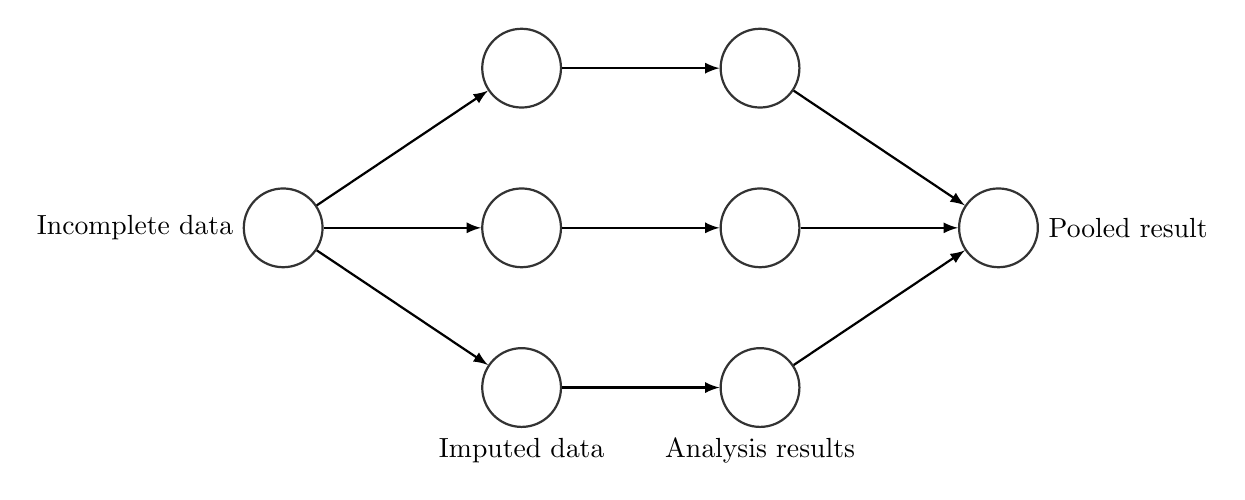
\begin{tikzpicture}
	\tikzstyle{main}=[circle, minimum size = 10mm, thick, draw =black!80, node distance = 20mm]
\tikzstyle{connect}=[-latex, thick]
\node[main, fill = white!100] (data) [label=left:Incomplete data] { };
\node[main] (mids) [right=of data] { };
\node[main] (mids2) [above=10mm of mids] { };
\node[main] (mids3) [below=10mm of mids,label=below:Imputed data] { };
\node[main] (mira) [right=of mids] {};
\node[main] (mira2) [above=10mm of mira] { };
\node[main] (mira3) [below=10mm of mira,label=below:Analysis results] { };
\node[main, fill = white!100] (mipo) [right=of mira,label=right:Pooled result] { };
\path (data) edge [connect] (mids)
      (data) edge [connect] (mids2)
      (data) edge [connect] (mids3)
      (mids) edge [connect] (mira)
      (mids2) edge [connect] (mira2)
      (mids3) edge [connect] (mira3)
		  (mira) edge [connect] (mipo)
		  (mira2) edge [connect] (mipo)
		  (mira3) edge [connect] (mipo);
\end{tikzpicture}}
\caption{Scheme of the main steps in multiple imputation ($m = 3$). Adapted from \citep[\S~1.4.1]{buur18}.}
\end{figure}

Missing data in $Y$ is `imputed' (i.e., filled in) $m$ times. The imputed data is combined with observed data $Y_{obs}$ to create $m$ completed data sets. On each completed data set, the analysis of scientific interest (or `complete data model') is performed. The quantity of scientific interest (e.g., a regression coefficient) is denoted with $Q$. Since $Q$ is estimated on each completed data set, $m$ separate $\hat{Q}$ values are obtained. These $m$ values are combined into a single pooled estimate $\bar{Q}$.

This note focusses on the algorithmic properties of the imputation step. The algorithm employed within this step has an iterative nature. That is, before drawing $m$ imputed values for each missing data point in $Y_{mis}$, a `chain' of potential values is considered. Each of the $m$ chains starts with an initial value, drawn randomly from $Y_{obs}$. The chains are terminated after a predefined number of iterations. Only the ultimate value that a chain lands on is imputed, and hence used in the next steps (analysis and pooling). The collection of values (or summary statistics) across iterations of each of the $m$ imputations will be referred to as an `imputation chain'. 

% "Let Q denote the quantity of scientific interest (e.g., a regression coefficient)." \cite[p.~4]{mice}.
% "Let Y denote the n x p matrix containing the data values on p variables for all n units in the sample. We define the response indicator R as an n x p 0-1 matrix. The elements of Y and R are denoted by y i j and r i j , respectively, where i = 1 , ... , n and j = 1 , ... , p . If y i j is observed, then r i j = 1 , and if y i j is missing, then r i j = 0 ." ... The observed data are collectively denoted by Y o b s . The missing data are collectively denoted as Y m i s , and contain all elements y i j where r i j = 0 . When taken together Y = ( Y o b s , Y m i s ) contain the hypothetically complete data." \cite[par.~2.2]{buur18}
% The data are said to be MCAR if Pr ( R = 0 | Y o b s , Y m i s , $\psi$ ) = Pr ( R = 0 | $\psi$ ) (2.1) so the probability of being missing depends only on some parameters $\psi$ , the overall probability of being missing. The data are said to be MAR if Pr ( R = 0 | Y o b s , Y m i s , $\psi$ ) = Pr ( R = 0 | Y o b s , $\psi$ ) (2.2) so the missingness probability may depend on observed information, including any design factors. Finally, the data are MNAR if Pr ( R = 0 | Y o b s , Y m i s , $\psi$ ) (2.3) does not simplify, so here the probability to be missing also depends on unobserved information, including Y m i s itself. \cite[par.~2.2]{buur18}

% Also introduce: 
% 
% - Terminology (MCAR, MAR, MNAR)?
% 
% - Blue points are observed, the red points are imputed?

%% -- Theoretical Background ---------------------------------------------------------------
\subsection{Theoretical Background} \label{sec:background}

The methodology for diagnosing convergence of multiple imputation algorithms has not been systematically studied \cite{buur18}. Yet, reference manuals of promiment MI software do mention the importance of evaluating algorithmic convergence (e.g., \cite[p.XYZ]{mice}, XYZ, XYZ). This section provides a brief review of how convergence is defined in the context of iterative algorithmic procedures, what diagnostic tools are available, and which of these may be applicable to MI algorithms. 




\textbf{Explain the measures that I'm investigating here. R hat is ... Auto-correlation is... How are they computed? What do they say? How are they computed on MI data? Looking at imputation chains. 
Explain that there is no baseline to compare the measures with. Only current convergence check is to visually inspect trace plots. (But in the trace-plots convergence seems immediate).}



\textbf{What is convergence in general?}

We can never be certain of convergence, therefore convergence diagnostics evaluate signs of non-convergence \citep{hoff09}. % In general: "In general, you cannot know for sure if your chain has converged. But sometimes you can know if your chain has not converged, so we at least check for this latter possibility" \cite[p.~101]{hoff09}
Convergence has two components \textbf{[look up source!!!]}: mixing between chains and stability over iterations within chains. Ideally, both components will be satisfied: there are no trends within chains, and the chains intermingle such that the only difference between the chains is caused by the randomness induced by the algorithm. Diagnose non-convergence in the mixing sense: $\widehat{R}$. Diagnose non-convergence in the stability sense: auto-correlation (AC). Also, it is possible to compute MC errors, or the Geweke statistic \citep{XYZ}. All of these methods evaluate the convergence of univariate scalars of interest (e.g., chain mean or chain variance). The convergence of multivariable statistics (i.e. relations between such scalars) may be evaluated via the eigenvector decomposition method proposed by McKay \citep{XYZ}. These three methods, however, are outside of the scope of this study. Here, the focus is mainly on $\widehat{R}$.

% "In order to converge to a stationary distribution, a Markov chain needs to satisfy three important properties (Roberts 1996; Tierney 1996): irreducible, the chain must be able to reach all interesting parts of the state space; aperiodic, the chain should not oscillate between different states; recurrence, all interesting parts can be reached infinitely often, at least from almost all starting points. Do these properties hold for the MICE algorithm? Irreducibility is generally not a problem since the user has large control over the interesting parts of the state space. This flexibility is actually the main rationale for FCS instead of a joint model. Periodicity is a potential problem, and can arise in the situation where imputation models are clearly inconsistent. A rather artificial example of an oscillatory behavior occurs when Y 1 is imputed by Y 2 $\beta$ + $\epsilon$  1 and Y 2 is imputed by - Y 1 $\beta$ + $\epsilon$  2 for some fixed, nonzero $\beta$ . The sampler will oscillate between two qualitatively different states, so the correlation between Y 1 and Y 2 after imputing Y 1 will differ from that after imputing Y 2 . In general, we would like the statistical inferences to be independent of the stopping point. A way to diagnose the ping-pong problem, or order effect, is to stop the chain at different points. The stopping point should not affect the statistical inferences. The addition of noise to create imputations is a safeguard against periodicity, and allows the sampler to "break out" more easily. Non-recurrence may also be a potential difficulty, manifesting itself as explosive or non-stationary behavior. For example, if imputations are made by deterministic functions, the Markov chain may lock up. Such cases can sometimes be diagnosed from the trace lines of the sampler. See Section 6.5.2 for an example. As long as the parameters of imputation models are estimated from the data, non-recurrence is mild or absent. The required properties of the MCMC method can be translated into conditions on the eigenvalues of the matrix of transition probabilities (MacKay 2003, 372-73). The development of practical tools that put these conditions to work for multiple imputation is still an ongoing research problem." \cite[par.~4.5]{buur18}

The potential scale reduction factor $\widehat{R}$ tells us by how much the variance of an estimate could be shrunken down, if the chains were to be infinitely long \cite{gelm92}. That then informs us about how dependent the chains are on the starting values. If there is no dependence on the initial values anymore, the chains have converged (in the mixing sense of the word). $\widehat{R}$ is then equal to one. The conventional acceptable threshold was $\widehat{R} < 1.2$. More recently, \cite{veht19} proposed a more stringent threshold: $\widehat{R} < 1.01$. 

We can apply $\widehat{R}$ to the mean (or to the first two moments) of the variables of interest. $\widehat{R}$ is defined by \cite{veth19} as follows: % The scalar summary of interest in this study is the average of the imputed values per variable. %As recommended by \cite{veht19} $\widehat{R}$ is computed as .... to be able to detect ... in the tails of the distribution. \cite[p.~5]{veth19}

\textbf{REPHRASE: In the equations below, $N$ is the number of draws per chain, $M$ is the number of chains, and $S = MN$ is the total number of draws from all chains. For each scalar summary of interest $\theta$, we compute $B$ and $W$, the between- and within-chain variances:}

\begin{align*}
``B&=\frac{N}{M-1} \sum_{m=1}^{M}\left(\bar{\theta}^{(\cdot m)}-\bar{\theta}^{(\cdot \cdot)}\right)^{2}, \text { where } \bar{\theta}^{(\cdot m)}=\frac{1}{N} \sum_{n=1}^{N} \theta^{(n m)}, \quad \bar{\theta}^{(\cdot \cdot)}=\frac{1}{M} \sum_{m=1}^{M} \bar{\theta}^{(\cdot m)} \\
W&=\frac{1}{M} \sum_{m=1}^{M} s_{j}^{2},  \text { where } s_{m}^{2}=\frac{1}{N-1} \sum_{n=1}^{N}\left(\theta^{(n m)}-\bar{\theta}^{(\cdot m)}\right)^{2}". \text{ \cite[p.~5]{veht19}} 
\end{align*}


The proportion of within chain variance $W$ against the weighted average of $B$ and $W$, $\widehat{\operatorname{var}}^{+}$ tells us how much variance of $\theta$ could be shrunken down if $N\to\infty$. $\widehat{\operatorname{var}}^{+}$ is computed as follows: %over-estimates the marginal posterior variance of the estimand, $\theta$. 

\begin{equation*}
\widehat{\operatorname{var}}^{+}(\theta | y)=\frac{N-1}{N} W+\frac{1}{N} B.
\end{equation*}

The potential scale reduction factor $\widehat{R}$ is obtained as:

\begin{equation*}
\widehat{R}=\sqrt{\frac{\widehat{\operatorname{var}}^{+}(\theta | y)}{W}}.
\end{equation*}

High $\widehat{R}$ would indicate .... low $\widehat{R}$ values indicate ....

The second component of convergence ... interpreted as stability over iterations, or non-recurring. Non-recurrence can be evaluated with auto-correlation. Auto-correlation shows how dependent subsequent draws of an imputation chain are on the previous value. If there is a lot of dependence, draws at e.g. iteration five are significantly correlated with the value of the first draw. A high auto-correlation indicates dependence within chains. The magnitude of the AC can be interpreted qualitatively, or compared to the critical value of a \textbf{XYZ} distribution with \textbf{XYZ} degrees of freedom.

\textbf{Convergence of MI}

The convergence properties of multiple imputation algorithms lack scientific consensus \citep{taka17}. A review by \citep{murr18}  and some default MICE techniques might not converge to stable distributions at all \citep{murr18}. Convergence diagnostics for MI methods have not been systematically studied \citep{buur18}.  Moreover, 
A fundamental assumption of MICE is convergence of the algorithm. MICE is a type of Markov chain Monte Carlo (MCMC) algorithm. In general, the validity of inference resulting from MCMC algorithms is threatened by non-convergence. Hence we use convergence diagnostics to flag non-convergence. But it is not known whether conventional convergence diagnostics for MCMC methods work on MI data.

$\widehat{R}$ may not be an appropriate diagnostic to evaluate MI data because it assumes over-dispersed initial values. This means that the initial values of the $m$ imputation chains are `far away' from the distribution that the chains are converging to. In the \pkg{mice} algorithm, initial values are chosen randomly from the observed data. Therefore, we cannot be certain that the initial values are over-dispersed. %The initial parameter value is noodzakelijk. Daarom is het lastig om in MI that starten vanuit overdisp state. 


% Starting values of MICE chains: "For each j, fill in starting imputations $Y^0_j$ by random draws from $Y^{obs}_j$." \cite[\S~4.5.2]{buur18} before for loops over variables and imputations, see \url{https://stefvanbuuren.name/fimd/sec-FCS.html#def:mice}

Without over-dispersed initial states, $\widehat{R}$ may falsely diagnose convergence \citep{broo98}. %would not be sensitive enough to flag non-convergence of MI algorithms: "if over-dispersion does not hold, $\sigma_+^2$ can be too low, which can lead to falsely diagnosing convergence." \cite[p~437]{broo98}. 
This suggests that $\widehat{R}$ would not be sensitive enough to flag non-convergence of MI algorithms. An empirical finding, however, shows that the opposite may be true: \cite{lace07} report $\widehat{R}$ values above the threshold of $\widehat{R} < 1.1$ after fifty iterations. %that $\widehat{R}$ will not be smaller than 1.1 before iteration number 50. Therefore, the aim is to replicate empirical finding Lacerda et al. 


\textbf{How is convergence checked now (current practice)?}

Conventional thresholds to diagnose non-convergence-- e.g., Gelman and Rubin's \citeyear{gelm92} statistic $\widehat{R} < 1.1$ --are not applicable on multiply imputed data \citep{lace07} \textbf{[Expand or remove Rhat here! Refer to future section?]}. Therefore, empirical researchers have to rely on visual inspection procedures that are theoretically equivalent to $\widehat{R}$ \citep{whit11} \textbf{[explain why this can still be appropriate, and numerical is not]}. Visually assessing convergence is not only challenging to the untrained eye, it might also be futile. 

% This research project consists of an investigation into algorithmic convergence of MI algorithms. I will replicate Lacerda et al.'s simulation study on $\widehat{R}$ \citep{lace07}, and develop novel guidelines for assessing convergence. Ideally, I will integrate several diagnostics (e.g., $\widehat{R}$, \emph{auto-correlation}, and \emph{simulation error}) into a single summary indicator to flag non-convergence.

\subsection{Simulation Hypothesis} \label{sec:hypothesis}

The aim is to evaluate whether the imputation procedure has converged. The primary research interest is in determining whether $\widehat{R}$ is an appropriate convergence diagnostic, and if so, which level of stringency suits MI data. \textbf{Or if there is a discrepancy between the visual and numeric inspection.}

The hypothesis of this simulation study is that $\widehat{R}$ will over-estimate non-convergence. \textbf{[Or use:] Hypothesis based on \cite{lace07} is that the conventional acceptable level of $\widehat{R}$ is too strict for MI data. We expect that the simulation diagnostics will indicate valid inference before $\widehat{R}$ will.}


% Also introduce:
% 
% - missingness mechanims, ignorability?
% % "The practical importance of the distinction between MCAR, MAR and MNAR is that it clarifies the conditions under which we can accurately estimate the scientifically interesting parameters without the need to know $\psi$" \cite[par.~2.2]{buur18}.
% 
% - Rubin's rules?
% 
% - FCS vs. JM?
% 

% \subsubsection{What is already implemented?}
% 
% - Trace-plots
% 
% \subsubsection{What is not yet implemented, but exists?}
% 
% - $\widehat{R}$, but too stringent (new) threshold, and assumption of over-dispersed initial values of imputation chains not met.
% % Potentially add something about updated (2019) version of $\widehat{R}$ and the new threshold of 1.01, see \citep{veht19}.
% 
% - Auto-correlation. Schafer (1997, p. 129) wrote on worst linear statistic. We could calculate the auto-correlation of that statistic to know that the algorithm converged elsewhere too. See autocorr function plot in SAS of worst linear function.
% % Worst linear function in SAS see \url{https://support.sas.com/documentation/cdl/en/statug/63033/HTML/default/viewer.htm#statug_mi_sect027.htm}.
% % Note: we're talking about missing data only, not the combined data (that autocorrelation is very high, as is the autocorrelation of deductively imputed values, like in the texp example). 
% % "Applications of MICE with lowly correlated data therefore inject a lot of noise into the system. Hence, the auto-correlation over t will be low, and convergence will be rapid, and in fact immediate if all variables are independent. Thus, the incorporation of noise into the imputed data has pleasant side-effect of speeding up convergence" \citep{buur18}, par. 4.5. 
% 
% - Sensitivity analysis: Run algorithm several times and compare results. 
% % "Imputers who do choose to use FCS should use flexible univariate models wherever possible and take care to assess apparent convergence of the algorithm, for example by computing traces of pooled estimates or other statistics and using standard MCMC diagnostics (Gelman et al., 2013, Chapter 11). It may also be helpful to examine the results of many independent runs of the algorithm with different initializations and to use random scans over the p variables to try to identify any convergence issues and mitigate possible order dependence" \cite[p.~19]{murr18}.
% 
% \subsubsection{What is not implemented, and NA?}
% 
% - $\widehat{R}$ threshold: Replicate simulation study and build a decision rule to solve the problem with $\widehat{R}$.
% % "The monitoring statistic was computed for mean monthly earnings at each iteration in chains of length k = 200. Since calculation of the statistic requires M parallel sequences, m = 5 such chains were constructed. This value of m was informed by the preferred choice given in the literature on multiple imputation. The monitoring statistic computed at each iteration is presented in Figures 15 to 17 for each of the three missingness mechanisms. The red vertical line denotes ten iterations" \cite[p.~49]{lace07}.
% 
% - Stability of the solution: Possibly use the slope of means over iterations too to see whether there is trending. Or apply PCA on the imputed data and if that (the eigenvalues?) stays the same we know that the means and variances are stable as well, see McKay (?). 
% 
% - MC error: MC error = SD/sqrt(number of iterations), where SD represents the variation across iterations. The MC error thus represents how much the means differ w.r.t. the iterations. MC error decreases as number of iterations increases. It should not be larger than 5\% of the sample standard deviation.

%% -- Methods ---------------------------------------------------------------

%%
%%
%%
%%

\section{Methods} \label{sec:methods}

To investigate convergence properties of the \pkg{mice} algorithm, different lenghts of imputation chains are considered. This simulation study considers 100 simulation conditions. Each condition has a different maximum number of iterations, varying between one and one-hundred iterations. In this study, 1000 simulation runs are performed for each of the 100 simulation conditions. \textbf{where for one through one hundred the Rhat and ... are calcuated.} The simulation set-up consists of several steps, summarized in the pseudo-code below. The complete \proglang{R} script of the simulation study is available on Github.

\begin{Code}
# pseudo-code of simulation 
simulate data 
for (number of simulation runs from 1 to 1000)
  for (number of iterations from 1 to 100)
    create missingness
    impute the missingness
    compute convergence diagnostics
    perform analysis
    pool results
    compute simulation diagnostics
aggregate convergence and simulation diagnostics
\end{Code}

\subsection{Data}
The simulated dataset is a finite population of $N=1000$. The data are simulated to solve a multiple linear regression complete data problem. The quantity of scientific interest is the estimated regression coefficient of predictor $X$ on outcome variable $Y$. The linear regression model is $Y \sim \beta_1 X + \beta_2 Z_1 + \beta_3 Z_2$, where $Y$ is the dependent variable, $X$ is an independent variable, and $Z_1$ and $Z_2$ are covariates. The data generating model of the predictors is a multivariate normal distribution with means structure $\mu$, and variance-covariance matrix $\Sigma$. 

\begin{align*}
\begin{pmatrix}X\\
Z_{1}\\
Z_{2}\\
\epsilon
\end{pmatrix} \sim  N
\begin{bmatrix}
\begin{pmatrix}
12\\
3\\
0.5\\
0
\end{pmatrix}\!\!,
\begin{pmatrix}
4 & 4 & 1.8 & 0\\
4 & 16 & 4.8 & 0\\
1.8 & 4.8 & 9 & 0\\
0 & 0 & 0 & 100
\end{pmatrix}
\end{bmatrix}\\[2\jot]
\end{align*}

Outcome variable $Y$ is subsequently calculated as $Y =  2X + .5Z_1 - Z_2 + \epsilon$.

\subsection{Amputation}
The complete data is the point of origin for all simulations. In each repetition of the simulation study, the complete data is `amputed' once. That is, the \pkg{mice} function \fct{ampute} in \proglang{R} is used to impose an MCAR missingness mechanism upon the data. The missingness is univariate, and the probability to be missing is the same for all variables, namely 20\%. This leaves 20\% of the rows completely observed. The resulting amputed data is equal for all simulation conditions in the same repetition.%"Furthermore, we generate three kinds of missingness proportions: 0.1, 0.5, and 0.9. Note that these values indicate the sampled proportion of incomplete cases in Y" \cite{schou18}.

\subsection{Imputation}
Missing data points are imputed with \pkg{mice} in \proglang{R}. All simulations are performed with imputation method 'norm' (Bayesian linear regression imputation), and five imputation chains ($m = 5$). The number of iterations is varied over simulations ('maxit' argument between 1 and 100). Each simulation condition (i.e., each number of iterations) is simulated 1000 times. Simulation and convergence diagnostics are aggregated over the 1000 MCMC simulations. 
% Missingness mechanism: "With MCAR missingness mechanisms, the probability to be missing is the same for all cases. This is a necessary simulation condition for evaluating the performance of imputation procedures. If an imputation method is not able to solve the problem (i.e. yield valid inference) under MCAR, the statistical properties of the procedure are not sound." (Vink, n.d., p. 4)
% "combine the m completed data inferences into a single inference following Rubin's (1987) rules (pp. 76-77)" \cite{schou18}.

\subsection{Convergence Diagnostics}
% Add ``post-processing steps (e.g. aggregation computations, summary statistics, regressions on the simulation results) used to transform simulation outputs to reported results''. %, see \url{http://jsterman.scripts.mit.edu/docs/Rahmandad-Sterman%20Simulation%20Reporting%20Standards3.30%20update.pdf}.

$\widehat{R}$ is computed within imputation chains: for each variable, each simulation condition, and each simulation. The maximum value across variables within the same simulation is reported. Maximum $\widehat{R}$ values per simulation condition are aggregated across simulations.

Auto-correlation (AC) is computed within imputation chains, as the correlation between $\theta$ at the $i^{th}$ iteration and $\theta$ at the $i+1^{th}$ iteration, where $\theta$ is a scalar summary of interest (i.e., chain means and chain variances). The AC of the variable with the highest absolute AC value is reported per simulation. These values are then averaged per simulation condition.


\subsection{Analysis}

Linear regression is performed using the \proglang{R} function \fct{lm}. The quantity of scientific interest $Q$ is the regression coefficient of $X$ on $Y$. $Q$ is estimated in each imputation, in each simulation condition, in each repetition. The $m = 5$ estimated regression coefficients $\hat{Q}$ are pooled according to Rubin's \citeyear{rubin87} rules with \pkg{mice} function \fct{pool}.

\subsection{Simulation diagnostics}
The simulation diagnostics are as recommended by \cite{buur18}. These comprise of average bias, average confidence interval width, and empirical coverage rate (coverage probability) across simulations. %"We expect that in accordance with Neyman (1934), at least 95 percent of the confidence intervals should contain the true population value, although some room for simulation error should be taken into account to counteract the finite nature of our simulations"\cite{schou18}.
We could also look at distributional characteristics, and plausibility of imputed values, see \cite{vinknd} (n.d.). For now, this is outside of the scope of this study. % Or use: Then evaluate the regular diagnostics of MI simulations, see Vink, n.d., and  convergence. Diagnostics include absolute bias of the estimated regression coefficient, confidence interval width, and empirical coverage rate across simulations. Convergence is evaluated with $\widehat{R}$, or potential scale reduction factor.

% Distributional characteristics: In practice, the distribution of the incomplete data may differ greatly from the observed data. Under anything but the MCAR assumption, this can be expected. When evaluating imputations, the distributional shapes should be checked and diagnostic evaluations should be performed (see Abayomi et al., 2008, for an detailed overview of diagnostic evaluation for multivariate imputations). When anomalies are found, and if the imputation method is valid, there should be an explanation, especially in the controlled environment of a properly executed simulation study. 

% Plausibility of the imputed values: Plausible imputations - imputations that could be real values if they had been observed - are not a necessary condition for obtaining valid inference. However, in practice, especially when the imputer and the analyst are different persons, plausibility of imputations may be a desired property. When evaluating imputation routines, the evaluator should mention whether the routine is prone to deliver implausible value

Bias is computed as the estimated regression coefficient after MI minus the true regression coefficient. Bias is averaged over all simulations with the same simulation condition.

Confidence interval width (CIW) is computed as the difference between the lower and upper bound of the 95\% confidence interval (CI95\%). The CI95\% bounds are computed as the estimated regression coefficient plus or minus (respectively) the pooled SE across imputations times 2.66 (the quantile of a t distribution with m-1 degrees of freedom). CIW is averaged over all simulations with the same simulation condition.

Coverage rate is computed as the proportion of simulations (with the same simulation condition) in which the true regression coefficient is between the bounds of the CI95\%. 



%% -- Results ---------------------------------------------------------------

%%
%%
%%
%%

\section{Results}


Figures \ref{fig:conv} and \ref{fig:sim} display results of the simulation study aggregated over 1000 repetitions. A subset of simulation conditions is presented in Table \ref{tab:results}. This section describes convergence diagnostics ($\widehat{R}$ and auto-correlation) and simulation diagnostics (bias, confidence interval width and coverage rate) separately.

\begin{figure}[h]
  \resizebox{\textwidth}{!}{ %notice the \resizebox{} command
        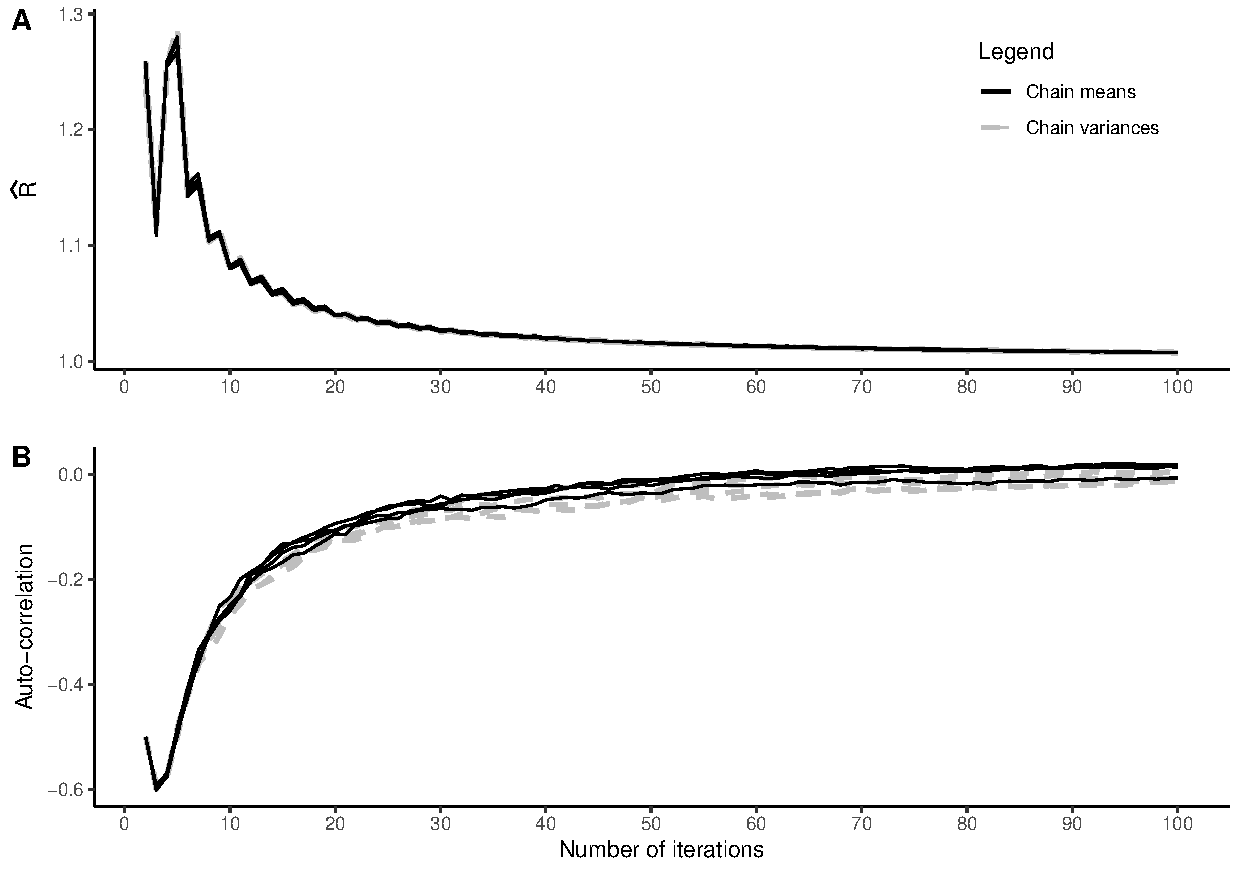
\includegraphics{Figures/convergence_diag.pdf}
  }
  \caption{Convergence diagnostics over 1000 MCMC simulations.}
    \label{fig:conv}
\end{figure}

\begin{figure}[h]
  \resizebox{\textwidth}{!}{ %notice the \resizebox{} command
        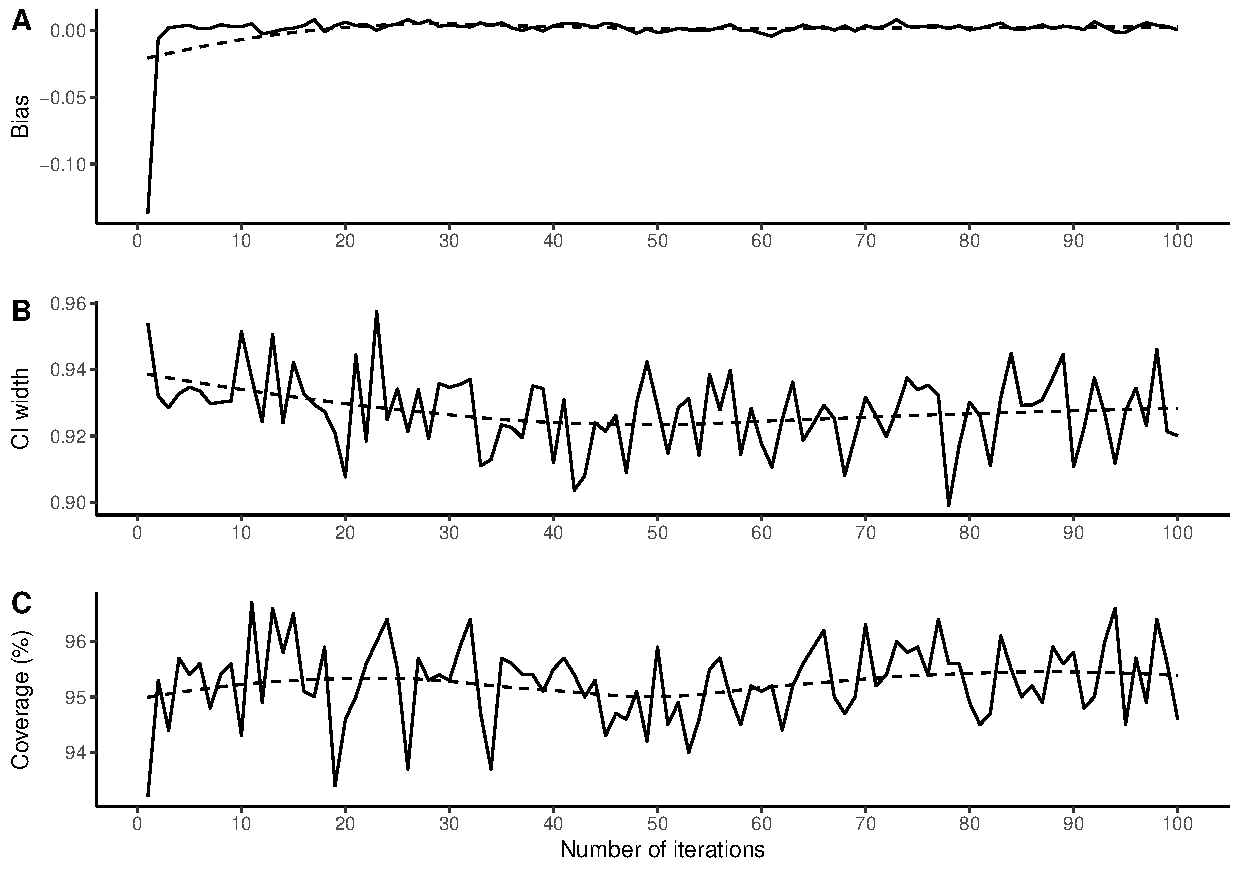
\includegraphics{Figures/simulation_diag.pdf}
  }
  \caption{Simulation diagnostics over 1000 MCMC simulations.}
    \label{fig:sim}
\end{figure}

% latex table generated in R 3.6.1 by xtable 1.8-4 package
% Wed Dec 04 18:16:11 2019
\begin{table}[ht]
\centering
\caption{Simulation and convergence diagnostics over 1000 MCMC simulations.} 
\label{tab:results}
\begin{tabular}{lrrrrrrr}
  \hline
It. & Bias & CI width & Cov. rate & $\widehat{R}_{mean}$ & $\widehat{R}_{var}$ & $AC_{mean}$ & $AC_{var}$ \\ 
  \hline
   1 & -0.137 & 0.954 & 0.932 & NA & NA & NA & NA \\ 
     2 & -0.006 & 0.932 & 0.953 & 1.650 & 1.632 & -0.500 & -0.500 \\ 
     3 & 0.002 & 0.929 & 0.944 & 1.314 & 1.306 & -0.660 & -0.659 \\ 
     4 & 0.003 & 0.933 & 0.957 & 1.461 & 1.457 & -0.733 & -0.735 \\ 
     5 & 0.004 & 0.935 & 0.954 & 1.475 & 1.472 & -0.705 & -0.706 \\ 
     6 & 0.001 & 0.934 & 0.956 & 1.258 & 1.256 & -0.656 & -0.646 \\ 
     7 & 0.002 & 0.930 & 0.948 & 1.265 & 1.269 & -0.591 & -0.585 \\ 
     8 & 0.004 & 0.930 & 0.954 & 1.181 & 1.178 & -0.495 & -0.516 \\ 
     9 & 0.003 & 0.931 & 0.956 & 1.187 & 1.187 & -0.442 & -0.459 \\ 
    10 & 0.003 & 0.952 & 0.943 & 1.141 & 1.140 & -0.403 & -0.423 \\ 
    15 & 0.002 & 0.942 & 0.965 & 1.100 & 1.100 & -0.276 & -0.289 \\ 
    25 & 0.005 & 0.934 & 0.955 & 1.057 & 1.057 & -0.143 & -0.159 \\ 
    50 & -0.002 & 0.929 & 0.959 & 1.027 & 1.026 & -0.053 & -0.075 \\ 
   100 & 0.000 & 0.920 & 0.946 & 1.013 & 1.013 & 0.022 & -0.017 \\ 
   \hline
\end{tabular}
\end{table}


%% --------------------------------
\subsection{Convergence diagnostics}

\textbf{$\widehat{R}$}. Steep decline up-to iteration twenty, then more gradual decrease up-to iteration forty, more or less stable after that. Conventional threshold $\widehat{R} < 1.2$ reached after seven or eight iterations, $\widehat{R} < 1.1$ after fourteen iterations for chain means and sixteen for chain variances, $\widehat{R} < 1.01$ not reached within the 100 iterations considered in this simulation study (see online appendix for the full table of results). \textbf{[REWRITE AS STORY, NOT JUST DATA.]} 

\textbf{Auto-correlation.} Within the 100 iterations considered in this study, the AC decreases steeply, before a slow increase. The lowest AC observed is -0.735 at four iterations. There appears to be a trend towards zero from four iterations upwards. Auto-correlation does not plateau completely. The average absolute maximum ACs are negative up to 77 iterations for chain means, and for chain variances all iterations considered here have negative ACs.

% \textbf{[Add simulation time (computational cost) to table? Add empirical SE of all diagnostics? Sample some random simulations and check distribution and plausibility of imputations? Use chain variance as scalar of interest for rhat and autocorrelation?]}

%% --------------------------------
\subsection{Simulation diagnostics}
\textbf{Bias.} From two iterations upwards, the average bias across repetitions is stable. Across iterations two to one hundred, bias fluctuates within a narrow range around zero. 
% Average bias is not zero because there is only one incomplete dataset to be imputed. Bias is a sample effect.

\textbf{Confidence interval width.} CIW does not show a clear trend across iterations. One might argue that there is some downward trending up-to thirthy to forty iterations. %After about twenty-five iterations the average CIW across all simulation conditions and repetitions is reached 0.928. 

\textbf{Coverage rate.} The coverage rate is more or less stable from two iterations upwards. On average, the coverage rate is somewhat higher than the expected nominal coverage of 95\% \cite{neym34}, namely 95.3\%. 

\textbf{add loess line to plots to see when it becomes a flat line. also, give some implications for these measures.}

%% -- Summary/conclusions/discussion -------------------------------------------
%%
%%
%%
%%

\section{Summary and discussion} \label{sec:summary}

\textbf{Summary.}
This note illustrates that conventional convergence diagnostics behave differently on MI data than other MCMC methods like Gibbs samplers in Bayesian analyses. The most recent recommended threshold for $\widehat{R}$ ($\widehat{R} < 1.01$) may be too stringent for MI data.

From the simulation diagnostics, it appears that as little as two iterations could be sufficient to draw \textbf{[valid inferences?]}. Convergence diagnostics $\widehat{R}$ and auto-correlation, however, indicate that convergence may only be reached after twenty or even forty iterations. 

\textbf{R hat below 1.}
$\widehat{R}$ could theoretically not be smaller than one, yet it occurred several times in this study (see online appendix XYZ). This can happen when the number of simulations is smaller than in `regular' MCMC processes [explain that fewer iterations is an advantage of MI, not a disadvantage compared to MCMC]. Therefore, the `$(n-1/n)$' [add equation number] correction factor can influence the estimated potential scale reduction factor. This downwards bias is in the opposite direction than expected: ``The mixture-of-sequences variance, $V$, should stabilize as a function of $n$. (Before convergence, we expect $\sigma^2$ to decrease with n, only increasing if the sequences explore a new area of parameter space, which would imply that the original sequences were not overdispersed for the particular scalar summary being monitored.)'' \cite[p~438]{broo98}.

% \url{https://discourse.mc-stan.org/t/rhat-1-as-low-as-9-94e-01-why/9252/3}

\textbf{Negative ACs.} Auto-correlation is dangerous when positive. These auto-correlations are negative. Still, we want the iterations to be stable and independent. Default maxit is five iterations now, should this be different? Are the 'waves' most pronounced at iteration 5? But why the dip??  

An implication of the observed dip in AC is that default maxit value of five iterations is the worst possible number of iterations.

\textbf{Future research.} We would like to have convergence measures for multivariable statistics (scalars?) of interest. This is, however, dependent on the complete data model. The eigenvector decomposition method proposed by McKay (?) should be implemented. I could not find any resources to apply this method and it is outside the scope of this thesis to investigate how this approach could be implemented. \textbf{[this paragraph is too negative, explain scope in intro instead.]}

%% -- Optional special unnumbered sections -------------------------------------

\section*{Computational details}

The results in this paper were obtained using \proglang{R}~3.6.1 \cite{R} with the \pkg{mice}~3.6.0.9000 package \cite{mice}. \proglang{R} itself and all packages used are available from the Comprehensive \proglang{R} Archive Network (CRAN) at \url{https://CRAN.R-project.org/}.


\section*{Acknowledgments}

This paper is written by the sole author (Hanne Oberman, BSc.), with guidance from Master thesis supervisors prof. dr. Stef van Buuren, and dr. Gerko Vink.

\textbf{LEAVING THIS HERE FOR REFERENCE, PLEASE REMOVE BEFORE HANDING IN}

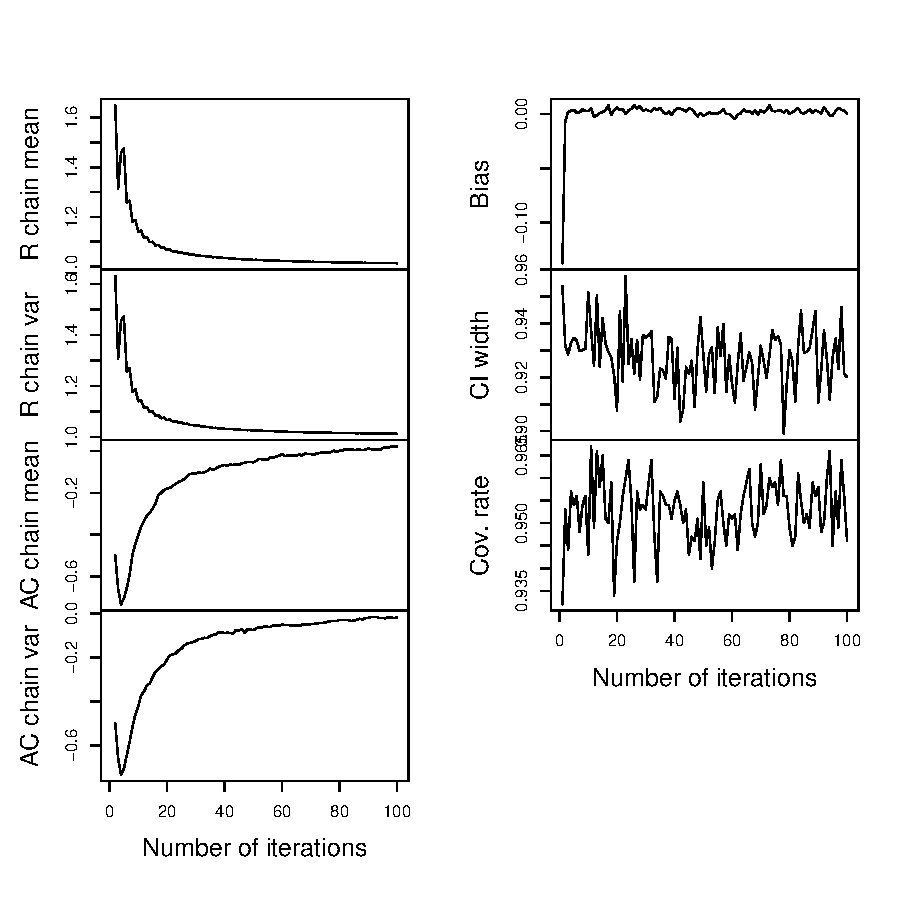
\includegraphics{NoteConvergence-003}

%% -- Bibliography -------------------------------------------------------------
%% - References need to be provided in a .bib BibTeX database.
%% - All references should be made with \cite, \citet, \citep, \citealp etc.
%%   (and never hard-coded). See the FAQ for details.
%% - JSS-specific markup (\proglang, \pkg, \code) should be used in the .bib.
%% - Titles in the .bib should be in title case.
%% - DOIs should be included where available.

\bibliography{ShinyMICE}


%% -- Appendix (if any) --------------------------------------------------------
%% - After the bibliography with page break.
%% - With proper section titles and _not_ just "Appendix".

\newpage

\begin{appendix}

\end{appendix}

%% -----------------------------------------------------------------------------


\end{document}
